% Created 2024-10-22 mar 11:33
% Intended LaTeX compiler: pdflatex
\documentclass[10pt]{article}
\usepackage[utf8]{inputenc}
\usepackage{lmodern}
\usepackage[T1]{fontenc}
\usepackage[top=1in, bottom=1.in, left=1in, right=1in]{geometry}
\usepackage{graphicx}
\usepackage{longtable}
\usepackage{float}
\usepackage{wrapfig}
\usepackage{rotating}
\usepackage[normalem]{ulem}
\usepackage{amsmath}
\usepackage{textcomp}
\usepackage{marvosym}
\usepackage{wasysym}
\usepackage{amssymb}
\usepackage{amsmath}
\usepackage[theorems, skins]{tcolorbox}
\usepackage[version=3]{mhchem}
\usepackage[numbers,super,sort&compress]{natbib}
\usepackage{natmove}
\usepackage{url}
\usepackage[cache=false]{minted}
\usepackage[strings]{underscore}
\usepackage[linktocpage,pdfstartview=FitH,colorlinks,
linkcolor=blue,anchorcolor=blue,
citecolor=blue,filecolor=blue,menucolor=blue,urlcolor=blue]{hyperref}
\usepackage{attachfile}
\usepackage{setspace}
\usepackage[spanish, ]{babel}
\date{}
\title{Consumo de petroleo y frecuencia del nombre Óscar}
\begin{document}

\maketitle
\section*{Datos}
\label{sec:org2ddb80d}

Ejemplo obtenido de
\url{https://tylervigen.com/spurious/correlation/8118\_popularity-of-the-first-name-oscar\_correlates-with\_petroluem-consumption-in-greece}

Datos anuales. Muestra: 1980--2022

\textbf{Consumo de petroleo en Grecia} \texttt{ConsumoPetroleo}

\begin{description}
\item[{Título detallado de la variable}] Volume of petroluem consumption consumed in Greece in millions of barrels per day
\item[{Fuente}] \href{https://www.eia.gov/international/data/world}{Energy Information Administration}
\end{description}

\textbf{Popularidad del nombre Óscar en EEUU} \texttt{FrecuenciaOscar}

\begin{description}
\item[{Título detallado de la variable}] Babies of all sexes born in the US named Óscar
\item[{Fuente}] \href{https://www.ssa.gov/oact/babynames/index.html}{US Social Security Administration}
\end{description}


\begin{minted}[frame=lines,fontsize=\scriptsize,linenos=]{r}
open NombreOscarYConsumoDePetroleo.gdt
\end{minted}

\begin{minted}[frame=lines,fontsize=\scriptsize,linenos=]{r}
gnuplot ConsumoPetroleo FrecuenciaOscar  --time-series --with-lines --output="PetroleoOscar.png"
\end{minted}

\begin{center}
\begin{tabular}{l}
\begin{center}
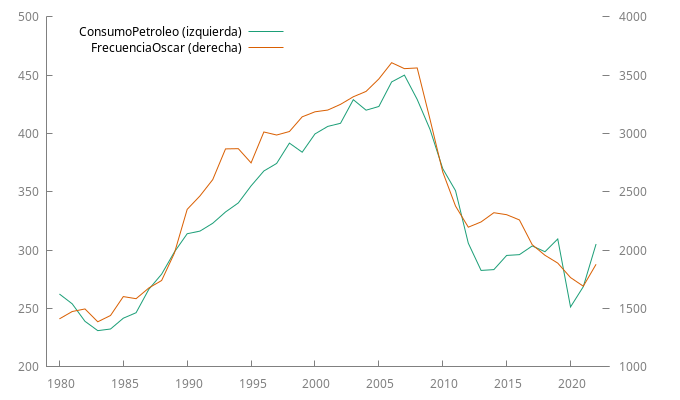
\includegraphics[width=.9\linewidth]{./NombreOscarYConsumoDePetroleo/PetroleoOscar.png}
\end{center}\\
\end{tabular}
\end{center}


\begin{itemize}
\item Ficheros \url{https://github.com/mbujosab/EconometriaAplicada-SRC/tree/main/Ejercicios}
\begin{itemize}
\item Versión en \href{https://github.com/mbujosab/EconometriaAplicada-SRC/blob/main/NombreOscarYConsumoDePetroleo.pdf}{pdf}
\item Datos: \url{NombreOscarYConsumoDePetroleo.gdt}
\item Guión de gretl: \url{NombreOscarYConsumoDePetroleo.inp}
\end{itemize}
\end{itemize}
\section*{Datos en nivel del consumo de petroleo en Grecia}
\label{sec:org1e80a49}
\subsection*{Gráfico de la serie temporal y su correlograma}
\label{sec:org54b7057}

\begin{minted}[frame=lines,fontsize=\scriptsize,linenos=]{r}
gnuplot ConsumoPetroleo --time-series --with-lines --output="consumoPetroleo.png"
corrgm ConsumoPetroleo 9 --plot="consumoPetroleoACF-PACF.png"
\end{minted}


\begin{center}
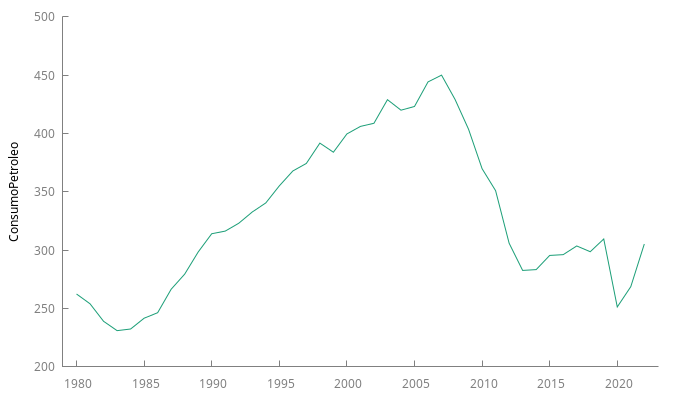
\includegraphics[width=0.5\textwidth]{./NombreOscarYConsumoDePetroleo/consumoPetroleo.png}
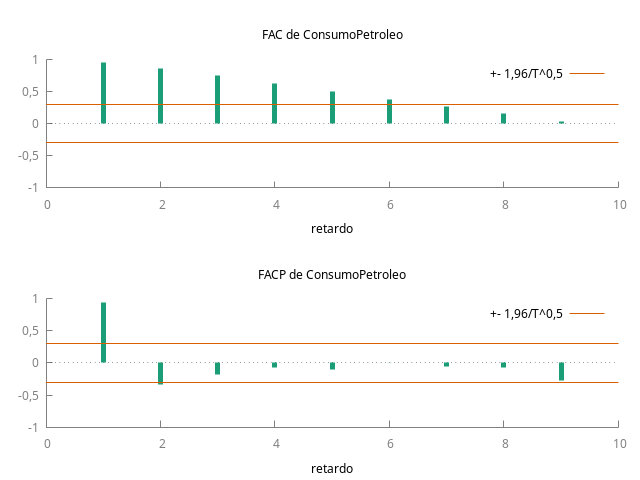
\includegraphics[width=0.4\textwidth]{./NombreOscarYConsumoDePetroleo/consumoPetroleoACF-PACF.png} 
\end{center}
\subsection*{Estimación de un primer modelo univariante para la serie de consumo de petroleo}
\label{sec:orgfa116c6}

\begin{minted}[frame=lines,fontsize=\scriptsize,linenos=]{r}
ARMApetroleo <- arima 1 0 1 ; ConsumoPetroleo
\end{minted}


\begin{verbatim}
Evaluaciones de la función: 41
Evaluaciones del gradiente: 14

ARMApetroleo:
ARMA, usando las observaciones 1980-2022 (T = 43)
Estimado usando AS 197 (MV exacta)
Variable dependiente: ConsumoPetroleo
Desviaciones típicas basadas en el Hessiano

             coeficiente   Desv. típica     z      valor p 
  ---------------------------------------------------------
  const      313,739        39,2711        7,989   1,36e-15 ***
  phi_1        0,930826      0,0477685    19,49    1,44e-84 ***
  theta_1      0,289746      0,135530      2,138   0,0325   **

Media de la vble. dep.  329,9135   D.T. de la vble. dep.   65,44053
Media de innovaciones   1,463908   D.T. innovaciones       17,36101
R-cuadrado              0,928461   R-cuadrado corregido    0,926717
Log-verosimilitud      -185,0353   Criterio de Akaike      378,0707
Criterio de Schwarz     385,1155   Crit. de Hannan-Quinn   380,6686

                       Real Imaginaria     Módulo Frecuencia
  -----------------------------------------------------------
  AR
   Raíz  1           1,0743     0,0000     1,0743     0,0000
  MA
   Raíz  1          -3,4513     0,0000     3,4513     0,5000
  -----------------------------------------------------------

ARMApetroleo guardado
\end{verbatim}

\begin{minted}[frame=lines,fontsize=\scriptsize,linenos=]{r}
series res1petroleo = $uhat
corrgm res1petroleo
\end{minted}


\begin{verbatim}
Función de autocorrelación para res1petroleo
***, ** y * indica significatividad a los niveles del 1%, 5% y 10%
utilizando la desviación típica 1/T^0,5

 RETARDO    FAC          FACP         Estad-Q. [valor p]

    1   0,0578        0,0578          0,1541  [0,695]
    2   0,1870        0,1843          1,8052  [0,406]
    3   0,1131        0,0972          2,4237  [0,489]
    4   0,0677        0,0264          2,6511  [0,618]
    5  -0,0189       -0,0630          2,6693  [0,751]
    6  -0,0371       -0,0659          2,7412  [0,841]
    7  -0,0590       -0,0547          2,9286  [0,892]
    8   0,2206        0,2638 *        5,6184  [0,690]
\end{verbatim}
\subsection*{Estimación de un segundo modelo univariante para la serie de consumo de petroleo}
\label{sec:org63f7bab}

\begin{minted}[frame=lines,fontsize=\scriptsize,linenos=]{r}
ARIpetroleo <- arima 1 1 0 --nc ; ConsumoPetroleo
\end{minted}


\begin{verbatim}
Evaluaciones de la función: 12
Evaluaciones del gradiente: 3

ARIpetroleo:
ARIMA, usando las observaciones 1981-2022 (T = 42)
Estimado usando AS 197 (MV exacta)
Variable dependiente: (1-L) ConsumoPetroleo
Desviaciones típicas basadas en el Hessiano

             coeficiente   Desv. típica     z     valor p
  -------------------------------------------------------
  phi_1       0,334680       0,151047     2,216   0,0267  **

Media de la vble. dep.  1,020476   D.T. de la vble. dep.   18,74413
Media de innovaciones   0,981800   D.T. innovaciones       17,53257
R-cuadrado              0,930469   R-cuadrado corregido    0,930469
Log-verosimilitud      -179,9453   Criterio de Akaike      363,8907
Criterio de Schwarz     367,3660   Crit. de Hannan-Quinn   365,1645

                       Real Imaginaria     Módulo Frecuencia
  -----------------------------------------------------------
  AR
   Raíz  1           2,9879     0,0000     2,9879     0,0000
  -----------------------------------------------------------

ARIpetroleo guardado
\end{verbatim}

\begin{minted}[frame=lines,fontsize=\scriptsize,linenos=]{r}
series res2petroleo = $uhat
corrgm res2petroleo
\end{minted}


\begin{verbatim}
Función de autocorrelación para res2petroleo
***, ** y * indica significatividad a los niveles del 1%, 5% y 10%
utilizando la desviación típica 1/T^0,5

 RETARDO    FAC          FACP         Estad-Q. [valor p]

    1  -0,0280       -0,0280          0,0354  [0,851]
    2   0,0692        0,0685          0,2567  [0,880]
    3   0,0756        0,0798          0,5278  [0,913]
    4   0,0412        0,0414          0,6102  [0,962]
    5  -0,0247       -0,0332          0,6406  [0,986]
    6  -0,0681       -0,0831          0,8788  [0,990]
    7  -0,0347       -0,0433          0,9423  [0,996]
    8   0,2664  *     0,2839 *        4,8001  [0,779]
\end{verbatim}
\section*{Datos en nivel de la popularidad del nombre Óscar en EEUU}
\label{sec:org112ee2b}
\subsection*{Gráfico de la serie temporal y su correlograma}
\label{sec:org398dc7a}

\begin{minted}[frame=lines,fontsize=\scriptsize,linenos=]{r}
gnuplot FrecuenciaOscar --time-series --with-lines --output="consumoOscar.png"
corrgm FrecuenciaOscar --plot="consumoOscarACF-PACF.png"
\end{minted}


\begin{center}
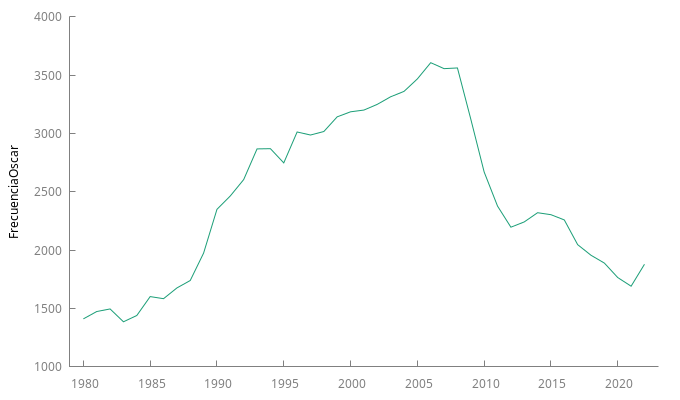
\includegraphics[width=0.5\textwidth]{./NombreOscarYConsumoDePetroleo/consumoOscar.png} 
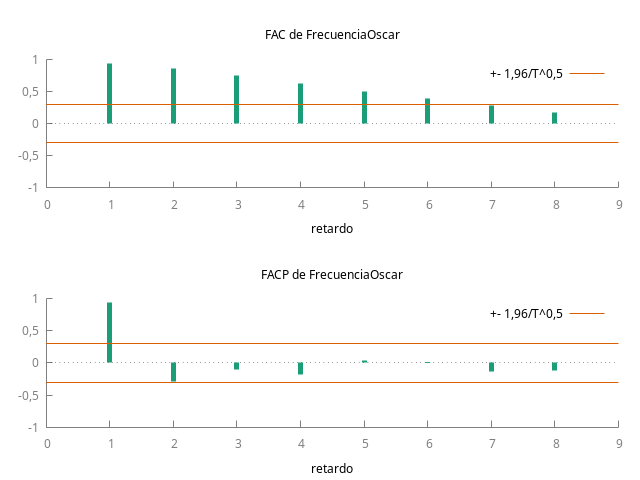
\includegraphics[width=0.4\textwidth]{./NombreOscarYConsumoDePetroleo/consumoOscarACF-PACF.png} 
\end{center}
\subsection*{Estimación de un primer modelo univariante para la serie de popularidad del nombre Óscar}
\label{sec:orgf709119}

\begin{minted}[frame=lines,fontsize=\scriptsize,linenos=]{r}
ARMAoscar <- arima 1 0 1 ; FrecuenciaOscar
\end{minted}


\begin{verbatim}
Evaluaciones de la función: 37
Evaluaciones del gradiente: 15

ARMAoscar:
ARMA, usando las observaciones 1980-2022 (T = 43)
Estimado usando AS 197 (MV exacta)
Variable dependiente: FrecuenciaOscar
Desviaciones típicas basadas en el Hessiano

             coeficiente   Desv. típica     z       valor p 
  ----------------------------------------------------------
  const      2083,23       517,026         4,029   5,60e-05  ***
  phi_1         0,951550     0,0384860    24,72    5,82e-135 ***
  theta_1       0,567719     0,127542      4,451   8,54e-06  ***

Media de la vble. dep.  2443,651   D.T. de la vble. dep.   702,2265
Media de innovaciones   16,93553   D.T. innovaciones       138,9316
R-cuadrado              0,960578   R-cuadrado corregido    0,959616
Log-verosimilitud      -274,9813   Criterio de Akaike      557,9626
Criterio de Schwarz     565,0074   Crit. de Hannan-Quinn   560,5605

                       Real Imaginaria     Módulo Frecuencia
  -----------------------------------------------------------
  AR
   Raíz  1           1,0509     0,0000     1,0509     0,0000
  MA
   Raíz  1          -1,7614     0,0000     1,7614     0,5000
  -----------------------------------------------------------

ARMAoscar guardado
\end{verbatim}

\begin{minted}[frame=lines,fontsize=\scriptsize,linenos=]{r}
series res1Oscar = $uhat
corrgm res1Oscar
\end{minted}


\begin{verbatim}
Función de autocorrelación para res1Oscar
***, ** y * indica significatividad a los niveles del 1%, 5% y 10%
utilizando la desviación típica 1/T^0,5

 RETARDO    FAC          FACP         Estad-Q. [valor p]

    1   0,0528        0,0528          0,1285  [0,720]
    2   0,2011        0,1988          2,0367  [0,361]
    3   0,2208        0,2107          4,3958  [0,222]
    4  -0,0966       -0,1595          4,8584  [0,302]
    5  -0,0753       -0,1733          5,1471  [0,398]
    6   0,1358        0,1690          6,1122  [0,411]
    7  -0,0222        0,0998          6,1386  [0,524]
    8   0,1386        0,1208          7,2006  [0,515]
\end{verbatim}
\subsection*{Estimación de un segundo modelo univariante para la serie de popularidad del nombre Óscar}
\label{sec:org8450059}

\begin{minted}[frame=lines,fontsize=\scriptsize,linenos=]{r}
ARIoscar <- arima 1 1 0 --nc ; FrecuenciaOscar
\end{minted}


\begin{verbatim}
Evaluaciones de la función: 11
Evaluaciones del gradiente: 4

ARIoscar: ARIMA, usando las observaciones 1981-2022 (T = 42)
Estimado usando AS 197 (MV exacta)
Variable dependiente: (1-L) FrecuenciaOscar
Desviaciones típicas basadas en el Hessiano

             coeficiente   Desv. típica     z     valor p 
  --------------------------------------------------------
  phi_1       0,535976       0,129413     4,142   3,45e-05 ***

Media de la vble. dep.  11,14286   D.T. de la vble. dep.   166,6352
Media de innovaciones   7,336036   D.T. innovaciones       138,9468
R-cuadrado              0,961704   R-cuadrado corregido    0,961704
Log-verosimilitud      -266,9966   Criterio de Akaike      537,9932
Criterio de Schwarz     541,4685   Crit. de Hannan-Quinn   539,2670

                       Real Imaginaria     Módulo Frecuencia
  -----------------------------------------------------------
  AR
   Raíz  1           1,8658     0,0000     1,8658     0,0000
  -----------------------------------------------------------

ARIoscar guardado
\end{verbatim}

\begin{minted}[frame=lines,fontsize=\scriptsize,linenos=]{r}
series res2Oscar = $uhat
corrgm res2Oscar
\end{minted}


\begin{verbatim}
Función de autocorrelación para res2Oscar
***, ** y * indica significatividad a los niveles del 1%, 5% y 10%
utilizando la desviación típica 1/T^0,5

 RETARDO    FAC          FACP         Estad-Q. [valor p]

    1   0,0027        0,0027          0,0003  [0,986]
    2  -0,0436       -0,0436          0,0881  [0,957]
    3   0,2378        0,2385          2,7683  [0,429]
    4  -0,1974       -0,2158          4,6634  [0,324]
    5  -0,1357       -0,1103          5,5826  [0,349]
    6   0,1327        0,0768          6,4862  [0,371]
    7  -0,0229        0,0634          6,5140  [0,481]
    8   0,1196        0,1581          7,2920  [0,505]
\end{verbatim}
\section*{Contraste de cointegración}
\label{sec:orgdca7019}

\begin{minted}[frame=lines,fontsize=\scriptsize,linenos=]{r}
coint 2 ConsumoPetroleo FrecuenciaOscar --test-down
\end{minted}

\begin{verbatim}
Etapa 1: contrastando la existencia de una raíz unitaria en ConsumoPetroleo

Contraste aumentado de Dickey-Fuller para ConsumoPetroleo
contrastar hacia abajo desde 2 retardos, con el criterio AIC
tamaño muestral 41
la hipótesis nula de raíz unitaria es: [a = 1]

  contraste con constante 
  incluyendo un retardo de (1-L)ConsumoPetroleo
  modelo: (1-L)y = b0 + (a-1)*y(-1) + ... + e
  valor estimado de (a - 1): -0,0697783
  estadístico de contraste: tau_c(1) = -1,6299
  valor p asintótico 0,4672
  Coef. de autocorrelación de primer orden de e: -0,087

Etapa 2: contrastando la existencia de una raíz unitaria en FrecuenciaOscar

Contraste aumentado de Dickey-Fuller para FrecuenciaOscar
contrastar hacia abajo desde 2 retardos, con el criterio AIC
tamaño muestral 41
la hipótesis nula de raíz unitaria es: [a = 1]

  contraste con constante 
  incluyendo un retardo de (1-L)FrecuenciaOscar
  modelo: (1-L)y = b0 + (a-1)*y(-1) + ... + e
  valor estimado de (a - 1): -0,0550591
  estadístico de contraste: tau_c(1) = -1,71873
  valor p asintótico 0,4218
  Coef. de autocorrelación de primer orden de e: -0,038

Etapa 3: regresión cointegrante

Regresión cointegrante - 
MCO, usando las observaciones 1980-2022 (T = 43)
Variable dependiente: ConsumoPetroleo

                   coeficiente  Desv. típica  Estadístico t  valor p 
  -------------------------------------------------------------------
  const            109,882       9,52812          11,53      1,90e-14 ***
  FrecuenciaOscar    0,0900421   0,00375080       24,01      9,21e-26 ***

Media de la vble. dep.  329,9135   D.T. de la vble. dep.   65,44053
Suma de cuad. residuos  11946,32   D.T. de la regresión    17,06967
R-cuadrado              0,933581   R-cuadrado corregido    0,931961
Log-verosimilitud      -181,9944   Criterio de Akaike      367,9888
Criterio de Schwarz     371,5112   Crit. de Hannan-Quinn   369,2878
rho                     0,538577   Durbin-Watson           0,872979

Etapa 4: contrastando la existencia de una raíz unitaria en uhat

Contraste aumentado de Dickey-Fuller para uhat
contrastar hacia abajo desde 2 retardos, con el criterio AIC
tamaño muestral 42
la hipótesis nula de raíz unitaria es: [a = 1]

  contraste sin constante 
  incluyendo 0 retardos de (1-L)uhat
  modelo: (1-L)y = (a-1)*y(-1) + e
  valor estimado de (a - 1): -0,461423
  estadístico de contraste: tau_c(2) = -3,49843
  valor p asintótico 0,03258
  Coef. de autocorrelación de primer orden de e: 0,094

Hay evidencia de una relación cointegrante si:
(a) La hipótesis de existencia de raíz unitaria no se rechaza para las variables individuales y
(b) La hipótesis de existencia de raíz unitaria se rechaza para los residuos (uhat) de la regresión cointegrante.
\end{verbatim}
\section*{Regresión del consumo de petroleo sobre la popularidad del nombre Óscar}
\label{sec:orgd2adbd9}
\subsection*{Primer modelo}
\label{sec:org99e815d}

\begin{minted}[frame=lines,fontsize=\scriptsize,linenos=]{r}
MCOpetroleoOscar <- ols ConsumoPetroleo 0 FrecuenciaOscar
modtest --normality --quiet
modtest --white --quiet
modtest --autocorr 1 --quiet
\end{minted}

\begin{verbatim}
Modelo 12: MCO, usando las observaciones 1980-2022 (T = 43)
Variable dependiente: ConsumoPetroleo

                   coeficiente  Desv. típica  Estadístico t  valor p 
  -------------------------------------------------------------------
  const            109,882       9,52812          11,53      1,90e-14 ***
  FrecuenciaOscar    0,0900421   0,00375080       24,01      9,21e-26 ***

Media de la vble. dep.  329,9135   D.T. de la vble. dep.   65,44053
Suma de cuad. residuos  11946,32   D.T. de la regresión    17,06967
R-cuadrado              0,933581   R-cuadrado corregido    0,931961
F(1, 41)                576,2946   Valor p (de F)          9,21e-26
Log-verosimilitud      -181,9944   Criterio de Akaike      367,9888
Criterio de Schwarz     371,5112   Crit. de Hannan-Quinn   369,2878
rho                     0,538577   Durbin-Watson           0,872979


Contraste de la hipótesis nula de distribución Normal:
Chi-cuadrado(2) = 1,252 con valor p 0,53467


Contraste de heterocedasticidad de White

Estadístico de contraste: TR^2 = 6,078609,
con valor p = P(Chi-cuadrado(2) > 6,078609) = 0,047868


Contraste de Breusch-Godfrey para autocorrelación de primer orden

Estadístico de contraste: LMF = 15,083365,
con valor p = P(F(1,40) > 15,0834) = 0,000377

Estadístico alternativo: TR^2 = 11,774602,
con valor p = P(Chi-cuadrado(1) > 11,7746) = 0,0006

Ljung-Box Q' = 11,8733,
con valor p = P(Chi-cuadrado(1) > 11,8733) = 0,000569
\end{verbatim}
\subsection*{Segundo modelo: regresión del consumo de petroleo sobre la popularidad del nombre Óscar con modelo de corrección de error AR1}
\label{sec:org8bdd913}

\begin{minted}[frame=lines,fontsize=\scriptsize,linenos=]{r}
MCOpetroleoOscarModeloErrorAR1 <- ar1 ConsumoPetroleo 0 FrecuenciaOscar
modtest --normality --quiet
\end{minted}

\begin{verbatim}
Realizando el cálculo iterativo de rho...

           ITERACIÓN   RHO        SCR
                   1      0,53858   8017,53
                   2      0,54713   8016,59
                   3      0,54824   8016,58
                   4      0,54839   8016,57
                   5      0,54841   8016,57

Modelo 14: Cochrane-Orcutt, usando las observaciones 1981-2022 (T = 42)
Variable dependiente: ConsumoPetroleo
rho = 0,548406

                   coeficiente  Desv. típica  Estadístico t  valor p 
  -------------------------------------------------------------------
  const            113,543      17,3686           6,537      8,31e-08 ***
  FrecuenciaOscar    0,0883312   0,00672160      13,14       4,24e-16 ***

Estadísticos basados en los datos rho-diferenciados:

Suma de cuad. residuos  8016,575   D.T. de la regresión    14,15678
R-cuadrado              0,954670   R-cuadrado corregido    0,953537
F(1, 40)                172,6961   Valor p (de F)          4,24e-16
rho                     0,093481   Durbin-Watson           1,760243

Estadísticos basados en los datos originales:

Media de la vble. dep.  331,5210   D.T. de la vble. dep.   65,36890


Contraste de la hipótesis nula de distribución Normal:
Chi-cuadrado(2) = 1,743 con valor p 0,41841
\end{verbatim}
\section*{Regresión en primeras diferencias}
\label{sec:orge20fc9f}
\subsection*{Primer modelo}
\label{sec:orgee14752}

\begin{minted}[frame=lines,fontsize=\scriptsize,linenos=]{r}
diff ConsumoPetroleo FrecuenciaOscar
MCOpetroleoOscar_en_Diff <- ols d_ConsumoPetroleo 0 d_FrecuenciaOscar
modtest --normality --quiet
modtest --white --quiet
modtest --autocorr 2 --quiet
\end{minted}

\begin{verbatim}
Modelo 16: MCO, usando las observaciones 1981-2022 (T = 42)
Variable dependiente: d_ConsumoPetroleo

                     coeficiente  Desv. típica  Estadístico t  valor p 
  ---------------------------------------------------------------------
  const               0,302707     2,40604         0,1258      0,9005  
  d_FrecuenciaOscar   0,0644152    0,0145806       4,418       7,40e-05 ***

Media de la vble. dep.  1,020476   D.T. de la vble. dep.   18,74413
Suma de cuad. residuos  9681,208   D.T. de la regresión    15,55732
R-cuadrado              0,327929   R-cuadrado corregido    0,311127
F(1, 40)                19,51752   Valor p (de F)          0,000074
Log-verosimilitud      -173,8411   Criterio de Akaike      351,6823
Criterio de Schwarz     355,1576   Crit. de Hannan-Quinn   352,9561
rho                    -0,041431   Durbin-Watson           2,000828


Contraste de la hipótesis nula de distribución Normal:
Chi-cuadrado(2) = 6,890 con valor p 0,03191


Contraste de heterocedasticidad de White

Estadístico de contraste: TR^2 = 2,712262,
con valor p = P(Chi-cuadrado(2) > 2,712262) = 0,257656


Contraste de Breusch-Godfrey para autocorrelación hasta el orden 2

Estadístico de contraste: LMF = 0,162094,
con valor p = P(F(2,38) > 0,162094) = 0,851

Estadístico alternativo: TR^2 = 0,355283,
con valor p = P(Chi-cuadrado(2) > 0,355283) = 0,837

Ljung-Box Q' = 0,314886,
con valor p = P(Chi-cuadrado(2) > 0,314886) = 0,854
\end{verbatim}
\subsection*{Segundo modelo: Regresión en primeras diferencias con intervención en el año 2020}
\label{sec:orgadbdf01}
Dado que hubo una caída muy acusada en el consumo de petroleo del año
20 debido al confinamiento por la Covid19 (\emph{circunstancia que no
afectó de manera particular a la popularidad del nombre "Óscar"}), el
siguiente modelo introduce una variable ficticia para el año 2020 (se
introduce en primeras diferencias como el resto de variables del
modelo).

\begin{minted}[frame=lines,fontsize=\scriptsize,linenos=]{r}
diff ConsumoPetroleo FrecuenciaOscar Covid
MCOpetroleoOscar_en_Diff_Covid <- ols d_ConsumoPetroleo 0 d_FrecuenciaOscar d_Covid
modtest --normality --quiet
modtest --white --quiet
modtest --autocorr 2 --quiet
\end{minted}

\begin{verbatim}
Modelo 18: MCO, usando las observaciones 1981-2022 (T = 42)
Variable dependiente: d_ConsumoPetroleo

                     coeficiente  Desv. típica  Estadístico t  valor p 
  ---------------------------------------------------------------------
  const                0,320457    2,07979          0,1541     0,8783  
  d_FrecuenciaOscar    0,0628222   0,0126104        4,982      1,33e-05 ***
  d_Covid            -36,2714      9,51424         -3,812      0,0005   ***

Media de la vble. dep.  1,020476   D.T. de la vble. dep.   18,74413
Suma de cuad. residuos  7052,862   D.T. de la regresión    13,44777
R-cuadrado              0,510389   R-cuadrado corregido    0,485281
F(2, 39)                20,32755   Valor p (de F)          8,96e-07
Log-verosimilitud      -167,1893   Criterio de Akaike      340,3786
Criterio de Schwarz     345,5917   Crit. de Hannan-Quinn   342,2894
rho                     0,100646   Durbin-Watson           1,708340


Contraste de la hipótesis nula de distribución Normal:
Chi-cuadrado(2) = 1,097 con valor p 0,57793


Contraste de heterocedasticidad de White

Estadístico de contraste: TR^2 = 2,155325,
con valor p = P(Chi-cuadrado(4) > 2,155325) = 0,707216


Contraste de Breusch-Godfrey para autocorrelación hasta el orden 2

Estadístico de contraste: LMF = 0,271314,
con valor p = P(F(2,37) > 0,271314) = 0,764

Estadístico alternativo: TR^2 = 0,607052,
con valor p = P(Chi-cuadrado(2) > 0,607052) = 0,738

Ljung-Box Q' = 0,464447,
con valor p = P(Chi-cuadrado(2) > 0,464447) = 0,793
\end{verbatim}
\section*{Preguntas}
\label{sec:orgc5baaf6}

\subsection*{Pregunta 1}
\label{sec:orgd3a3ca7}

Discuta de todas las formas posibles si las series temporales de
consumo de petroleo (\texttt{ConsumoPetroleo}) y popularidad del nombre Óscar
(\texttt{FrecuenciaOscar}) son estacionarias en media (i.e., son la
realización de procesos estocásticos estacionarios), usando para ello
los resultados de los apartados \hyperref[sec:org1e80a49]{Datos en nivel del consumo de petroleo en Grecia}, \hyperref[sec:org112ee2b]{Datos en nivel de la popularidad del nombre Óscar en EEUU} y
\hyperref[sec:orgdca7019]{Contraste de cointegración}.

(\hyperref[sec:orga953cfd]{Respuesta 1})
\subsection*{Pregunta 2}
\label{sec:org9c9b72f}

Discuta si las series temporales \texttt{ConsumoPetroleo} y \texttt{FrecuenciaOscar}
están cointegradas, a partir de los resultados del apartado \hyperref[sec:orgdca7019]{Contraste de cointegración}.

(\hyperref[sec:orgb9e4dcc]{Respuesta 2})
\subsection*{Pregunta 3}
\label{sec:org0f9a56b}

¿Contradice la \hyperref[sec:orge20fc9f]{Regresión en primeras diferencias} la posibilidad de que
están relacionados el consumo de petroleo en Grecia y la popularidad
del nombre de pila Oscar en los EEUU?

(\hyperref[sec:org014d2fe]{Respuesta 3})
\subsection*{Pregunta 4}
\label{sec:org8e2fed6}

Los listados de la \hyperref[sec:orgd2adbd9]{Regresión del consumo de petroleo sobre la popularidad del nombre Óscar} y la \hyperref[sec:orge20fc9f]{Regresión en primeras diferencias}
muestran los principales resultados obtenidos al estimar por MCO dos
modelos de regresión que relacionan las dos variables consideradas en
este ejercicio (dichos modelos están referidos como "\emph{primeros
modelos}").

Resuma y comente los resultados de estimación y diagnosis que le
parezcan más relevantes de esos dos primeros modelos en niveles y en
diferencias.

Si detecta alguna desviación del cumplimiento de las hipótesis
habituales, discuta sus consecuencias sobre las propiedades del
estimador MCO y sugiera alguna forma de tratarla.

(\hyperref[sec:org4f3f44d]{Respuesta 4})
\subsection*{Pregunta 5}
\label{sec:org516e60d}

Tanto en el caso de las regresiones en niveles como en el caso de las
regresiones en primeras diferencias, también se muestra los resultados
de un segundo modelo de regresión.

Explique en cada caso si ese segundo modelo responde a algún posible
tratamiento que haya indicado en la pregunta anterior y por qué (o si
dicho tratamiento no tiene nada que ver con lo que usted dijo). En
cualquier caso, señale (en cada caso) si considera que ese segundo
modelo es mejor o peor que el primero, y en qué aspectos.


(\hyperref[sec:orgfe4b59b]{Respuesta 5})
\subsection*{Pregunta 6}
\label{sec:org5ca64fb}

En la Sección \hyperref[sec:org1e80a49]{Datos en nivel del consumo de petroleo en Grecia}
aparecen dos modelos univariantes. Compare los resultados he indique
si alguno de ellos es preferible y por qué.

(\hyperref[sec:org756e936]{Respuesta 6})
\subsection*{Pregunta 7}
\label{sec:orge819da2}

En la Sección \hyperref[sec:org112ee2b]{Datos en nivel de la popularidad del nombre Óscar en EEUU} aparecen dos modelos univariantes. Compare los resultados he
indique si alguno de ellos es preferible y por qué.

(\hyperref[sec:orge819da2]{Pregunta 7})
\subsection*{Pregunta 8}
\label{sec:org8534066}

¿Cuáles de los modelos de más arriba considera aceptables? ¿O qué
mejoras sugeriría para ellos?

(\hyperref[sec:orgf9d3e51]{Respuesta 8})

\newpage
\section*{Respuestas}
\label{sec:org87a570a}

\subsection*{Respuesta 1}
\label{sec:orga953cfd}

Ambas series (\texttt{ConsumoPetroleo} y \texttt{FrecuenciaOscar}) parecen ser NO
estacionarias en media,
\begin{itemize}
\item Sus gráficos muestran una clara evolución de su nivel a lo largo de
la muestra (los primeros años ascendente y desde 2005 descendente).

\item Ambas funciones de autocorrelación (FAC) muestran persistencia (sus
coeficientes decrecen despacio y a un ritmo aproximadamente lineal);
y el primer coeficiente de la PACF está próximo a uno en ambos
casos.

\item \hyperref[sec:orgfa116c6]{Estimación de un primer modelo univariante para la serie de consumo de petroleo}: El modelo univariante estimado tiene una raíz AR
aproximadamente igual a \(1\).

\item \hyperref[sec:orgf709119]{Estimación de un primer modelo univariante para la serie de popularidad del nombre Óscar}: El modelo univariante estimado tiene
una raíz AR aproximadamente igual a \(1\).

\item \hyperref[sec:orgdca7019]{Contraste de cointegración}: Los test ADF calculados en las etapas 1
y 2 no rechazan la hipótesis (raíz unitaria) con p-valores
superiores al 0.4
\end{itemize}

(\hyperref[sec:orgd3a3ca7]{Pregunta 1})
\subsection*{Respuesta 2}
\label{sec:orgb9e4dcc}

Las conclusiones de las distintas etapas del test de cointegración son:
\begin{description}
\item[{Etapa 1}] El test ADF no rechaza que la serie \texttt{ConsumoPetroleo} sea
I(1) para niveles de significación inferiores al 40\% (p-valor
asintótico \texttt{0,4672}).
\item[{Etapa 2}] El test ADF no rechaza que la serie \texttt{FrecuenciaOscar} sea
I(1) para niveles de significación inferiores al 40\% (p-valor
asintótico \texttt{0,4218}).
\item[{Etapa 3}] En la regresión (cointegrante) de mortalidad sobre la
proporción de matrimonios eclesiásticos ambos parámetros (constante
y pendiente) resultan ser muy significativos, y el \(R^2\) está
próximo a 1.
\item[{Etapa 4}] El test ADF rechaza que los residuos de la regresión
cointegrante sean I(1) tanto al 10\% como al 5\% de significación
(p-valor asintótico \texttt{0,03258})
\end{description}

Consecuentemente, \uline{el test NO rechaza la cointegración de ambas
series} (\emph{en contra de lo que sugiere el sentido común}).

(\hyperref[sec:org9c9b72f]{Pregunta 2})
\subsection*{Respuesta 3}
\label{sec:org014d2fe}

\uline{La relación NO se desvanece al diferenciar los datos} para lograr la
estacionariedad; que es precisamente lo que cabe esperar cuando la
relación existe, pues si
$$
\boldsymbol{y}=\beta_1 \boldsymbol{1} + \beta_2 \boldsymbol{x} + \boldsymbol{u}
$$
Entonces también debe ser cierto que
$$
\nabla\boldsymbol{y}= \beta_2 \nabla\boldsymbol{x} + \nabla\boldsymbol{u}
$$

Sorprendentemente, en la \hyperref[sec:orge20fc9f]{Regresión en primeras diferencias} la
constante es NO significativa, la pendiente es muy significativa y el
\(R^2\) no es, en absoluto, despreciable (\texttt{R-cuadrado 0,327929}). Es
decir, \uline{la \hyperref[sec:orge20fc9f]{Regresión en primeras diferencias} no contradice la
posibilidad de que ambas variables estén relacionadas}.

\emph{Comentario y moraleja}: Pese a los resultados estadísticos, la
relación entre \texttt{ConsumoPetroleo} y \texttt{FrecuenciaOscar} es evidentemente
espuria (es imposible argumentar con algún fundamento que la
frecuencia del nombre Óscar en EEUU tenga ninguna influencia sobre el
consumo de petroleo en Grecia\ldots{} o viceversa). ¡Ojo con interpretar
los resultados estadísticos sin un mínimo espíritu crítico!

(\hyperref[sec:org0f9a56b]{Pregunta 3})
\subsection*{Respuesta 4}
\label{sec:org4f3f44d}

\begin{description}
\item[{Primer modelo para datos en nivel}] (\hyperref[sec:orgd2adbd9]{Regresión del consumo de petroleo sobre la popularidad del nombre Óscar}): Todos los
coeficientes son muy significativos. El ajuste del modelo, medido
por el valor del \(R^2\) es muy elevado. Los contrastes sobre los
residuos no rechazan la hipótesis nula de normalidad, pero si
rechazan la hipótesis de homocedasticidad y de autocorrelación.

En cuanto a la heterocedasticidad, sería conveniente estimar
indicando la opción de desviaciones típicas robustas, pues los
p-valores están mal calculados en presencia de
heterocedasticidad. Más importante es la presencia de
autocorrelación; dado que hay indicios de autocorrelación de orden 1
en los errores de ajuste, sería conveniente estimar el modelo
incorporando un modelo AR(1) para el error.

\item[{Primer modelo para datos en primeras diferencias}] (\hyperref[sec:orge20fc9f]{Regresión en primeras diferencias}): El único coeficiente significativo es la
pendiente (es decir, al diferenciar las series ha desaparecido la
relación entre ellas), y el ajuste del modelo, medido por el valor
del \(R^2\), es superior al 30\%. Los contrastes residuales rechazan
la hipótesis nula de normalidad, pero no rechazan las de
homoscedasticidad y ausencia de autocorrelación.

Si las perturbaciones no tienen distribución normal las estimaciones
no serán eficientes en el sentido máximo-verosímil (aunque sí en el
de Gauss-Markov) y la distribución de los estadísticos habituales
será distinta de la teórica bajo el supuesto de normalidad de las
perturbaciones (por ejemplo, los estadísticos de la \(t\) no tendrán
exactamente una distribución \emph{t} de student). En la práctica esto no
ocasiona un problema grave en general.
\end{description}

(\hyperref[sec:org8e2fed6]{Pregunta 4})
\subsection*{Respuesta 5}
\label{sec:orgfe4b59b}


\begin{description}
\item[{Segundo modelo para datos en nivel}] (\hyperref[sec:orgd2adbd9]{Regresión del consumo de petroleo sobre la popularidad del nombre Óscar}): El segundo modelo
corresponde a una regresión con modelo AR(1) para el error (tal y
como se sugería en la pregunta anterior). La estimación ha
convergido en 5 iteraciones, los parámetros son muy significativos y
el \(R^2\) ajustado es superior al del primer modelo. Tampoco en este
caso se rechaza la hipótesis de normalidad en los residuos del
ajuste. Todo ello sugiere que este segundo modelo sería ligeramente
superior al primero (\emph{si no fuera porque la relación es
evidentemente espuria y, por tanto, ninguno de estos modelos es
aceptable}).
\end{description}


\begin{description}
\item[{Segundo modelo para datos en primeras diferencias}] (\hyperref[sec:orge20fc9f]{Regresión en primeras diferencias}): El segundo modelo incluye un nuevo regresor
para captar la caída de consumo de petroleo del año 2020 debida al
confinamiento por la Covid19. Por tanto, esta modificación no tiene
nada que ver con lo indicado en la pregunta anterior.

No obstante, este modelo parece superior al primero. Los parámetros
correspondientes a \texttt{d\_FrecuenciaOscar} y \texttt{d\_Covid} son muy
significativos, el \(R^2\) ajustado es claramente superior y los
criterios de información han mejorado ligeramente (i.e., ahora toman
valores más bajos). Además, gracias a la intervención del año
atípico 2020, los residuos pasan todos los contrastes (incluido el
de normalidad).
\end{description}

(\hyperref[sec:org516e60d]{Pregunta 5})
\subsection*{Respuesta 6}
\label{sec:org756e936}

El primer modelo es un ARMA(\(1,1\)) con media distinta de cero, y los
tres parámetros estimados son muy significativos. El mayor
inconveniente es que la raíz autorregresiva es prácticamente \(1\). Dado
que hay una fuerte evidencia de que el proceso NO es estacionario en
media, es preferible diferenciar la serie e identificar un proceso
ARIMA.

El segundo modelo es un ARIMA(1,1,0) con media cero. Su principal
ventaja es que el modelo estimado corresponde a un proceso que (una
vez diferenciado) es invertible y estacionario (pues no tiene
polinomio MA, y el módulo de la raíz AR es \texttt{2,9879} \(>1\)). 

Pese a que tiene menos parámetros estimados, el ajuste y los criterios
de información son ligeramente mejores. Además, los p-valores de los
estadísticos Q de Ljung-Box son más elevados en este segundo modelo,
por lo que sus residuos tienen una mayor apariencia de "ruido
blanco". En resumen, este segundo modelo parece mejor que el primero.

(\hyperref[sec:org5ca64fb]{Pregunta 6})
\subsection*{Respuesta 7}
\label{sec:orgd3033cf}

Como en el caso anterior, el primer modelo es un ARMA(\(1,1\)) con media
distinta de cero, y los tres parámetros estimados son muy
significativos. De nuevo, el mayor inconveniente es que la raíz
autorregresiva es prácticamente \(1\). Dado que hay una fuerte evidencia
de que el proceso NO es estacionario en media, es preferible
diferenciar la serie e identificar un proceso ARIMA.


El segundo modelo es un ARIMA(1,1,0) con media cero. Su principal
ventaja es que el modelo estimado corresponde a un proceso que (una
vez diferenciado) es invertible y estacionario (pues no tiene
polinomio MA, y el módulo de la raíz AR es \texttt{1,8658} \(>1\)). 

Pese a que tiene menos parámetros estimados, el ajuste y los criterios
de información son ligeramente mejores. Además, los p-valores de los
estadísticos Q de Ljung-Box son más elevados en este segundo modelo,
por lo que sus residuos tienen una mayor apariencia de "ruido
blanco". En resumen, este segundo modelo parece mejor que el primero.

(\hyperref[sec:org5ca64fb]{Pregunta 6})
\subsection*{Respuesta 8}
\label{sec:orgf9d3e51}

\begin{description}
\item[{En cuanto a los modelos univariantes}] Como se ha dicho, para ambas
series, el segundo modelo es mejor que el primero. En ambos casos
corresponde a un proceso invertible y estacionario, el parámetro
estimado es significativo y (según los estadísticos Q de Ljung-Box)
los residuos parecen ruido blanco.

\item[{En cuanto a los modelos de regresión}] Los cuatro modelos intentan
modelizar una relación evidentemente espuria: nada tiene que ver la
popularidad del nombre Óscar en EEUU con el consumo de petroleo en
Grecia. Consecuentemente ninguna de estas regresiones ofrece un
modelo aceptable o, ni siquiera, razonable.
\end{description}

(\hyperref[sec:org8534066]{Pregunta 8})
\end{document}
